\chapter{Objektsysteme in Racket}
Racket ist ein Dialekt von Lisp, der auf Scheme basiert. Es ist jedoch keine rein funktionale Sprache, sondern unterstützt verschiedene Lisp-Dialekte und  Programmierparadigmen. 
%Damit gibt Racket Programmierern und Forschern die Werkzeuge, die sie benötigen, um neue Sprachen zu erkunden und zu entwickeln\cite{racketguide-dialects} und wird beispielsweise auch an der Universität Hamburg in der Forschung genutzt.

Racket wird an der Universität Hamburg in der Softwareentwicklungslehre genutzt, da es im Gegensatz zu Common Lisp sehr einstiegsfreundlich ist. Die Veranstaltungsteilnehmer lernen zum ersten Mal eine funktionale Sprache kennen und sollen einen möglichst einfachen Einstieg erhalten. Hierzu bietet Racket eine übersichtliche Syntax und eine plattformunabhängige Entwicklungsumgebung, die vergleichbare Fehlermeldungen liefert.

In Common Lisp wird die Syntax schnell sehr komplex und ist zudem abhängig von der Implementierung (teilweise sogar mit kostenpflichtigem Interpreter). Common Lisp hat zwei verschiedene Paketsysteme mit tausenden von Paketen, was ein schnelles Zurechtfinden in der Sprache nicht begünstigt. Es gibt keine dedizierte grafische Oberfläche, da Common Lisp für die Integration in Emacs, Vim etc. ausgelegt ist. Das bedeutet, dass Veranstaltungsteilnehmer sich anfangs mit der Integration der Sprache im Editor ihrer Wahl beschäftigen müssen, bevor sie überhaupt eine Zeile Code schreiben können. Nicht alle Interpreter von Common Lisp werden  für alle Betriebssysteme gewartet, wie zum Beispiel SBCL, der frei verfügbar und sehr performant ist, jedoch unter Windows nur gelegentlich gepflegt wird. Eine Ursachenermittlung von Fehlern ist nur unter hohem Aufwand durchführbar, da immer das verwendete Betriebssystem berücksichtigt werden muss. Zudem ist eine systemübergreifende grafische Ausgabe ohne weitere Pakete nicht vorgesehen. Dadurch werden Übungsaufgaben erschwert, bei denen das Ergebnis visualisiert werden kann oder muss, da die grafische Ausgabe vom Interpreter abhängig ist und die Teilnehmer zudem die entprechenden Pakete installieren müssten. 

Um Common Lisp zu lernen, wurde daher Scheme entwickelt. Analog zu BlueJ, einer Entwicklungsumgebung für das Lernen von objektorientierter Programmierung in Java, war DrScheme das Einsteigertool zu Common Lisp. Im Jahr 2010 wurde Scheme umbenannt zu Racket. Racket bildet einen guten Kompromiss für die Lehre, da es einen leicht verständlichen Einstieg in die Welt von Common Lisp bietet.
%----------------------

Die Syntax von Racket ist sehr ähnlich zu Common Lisp. Ausdrücke werden im Präfixnotation geschrieben, Kommentare mit einem Semikolon eingeleitet. Einige Standardfunktionen haben leicht abgewandelte Namen. So werden in Racket beispielsweise sowohl Funktionen als auch Variablen mit dem Schlüsselwort \texttt{define} definiert, anstelle von \texttt{defun}, \texttt{defvar} und \texttt{defparameter} in Common Lisp. Prädikate enden auf \texttt{?} (zum Beispiel \texttt{equal?}) und Methoden, die Variablen oder Objekte verändern auf \texttt{!} (zum Beispiel \texttt{set!}). Einer der größeren Unterschiede liegt in der Art, wie Makros definiert werden; darauf wird im Kapitel \ref{makros} noch näher eingegangen.

Racket unterstützt auch objektorientierte Programmierung auf zwei verschiedene Arten. Zunächst gibt es das Racket-Objektsystem. Racket-Klassen sind sehr ähnlich zu Klassen in Java, C\# oder den meisten objektorientierten Programmiersprachen. Ein Programm kann Klassen definieren, instanziieren, mit den erzeugten Objekten interagieren und Klassen erweitern. Besonders ist, dass Klassen auch wie Funktionswerte behandelt werden können. Es ist möglich, eine Klasse zur Laufzeit zu erweitern, eine Klasse an eine Funktion zu geben oder in einer Datenstruktur zu speichern und anschließend abzufragen \cite{neu-edu}. 

Zusätzlich gibt es den Racket-Dialekt Swindle, in dem das Common Lisp Object System (CLOS) implementiert ist. Im Gegensatz zum eingebauten Objektsystem von Racket bietet CLOS Funktionalitäten wie Mehrfachvererbung, Methodenkombination oder Ergänzungsmethoden. Durch die Implementierung als Metaobject-Protocol bietet es dem Programmierer zudem viel Freiheit bei der Erweiterung und Veränderung der Repräsentation von Klassen und Objekten.

Um ein Grundverständnis der beiden Objektsysteme zu erhalten, soll zunächst betrachtet werden, wie sie benutzt werden können. %Andschließend wird ein Blick auf die Implementierung beider Ansätze geworfen. Die Autoren des Buches ``The Art of the Metaobject Protocol''\cite{amop} vergleichen das Vorgehen sehr treffend mit eine Theateraufführung: Auf der Bühne (onstage) findet das Theaterstück statt - das Programm, oder etwas allgemeiner, das, was der Programmierer von der Sprache sieht. Hinter der Bühne (backstage) befindet sich die darunterliegende Implementierung, die die entprechenden Makros definiert und mit für den Programmierer nicht sichtbaren Objekten und Funktionen arbeitet. Wir wollen beide Ansätze erst ``onstage'' betrachten bevor wir einen Blick hinter die Kulissen werfen.

Der Fokus dieser Arbeit liegt auf der Implementierung von Mehrfachvererbung im Objektsystem von Racket. Natürlich bieten sowohl das Objektsystem von Racket als auch CLOS neben Vererbung auch noch viele weitere nützliche Funktionen und Eigenschaften; diese sind jedoch nicht zielführend für diese Arbeit und es würde eine eigene Ausarbeitung benötigen, sie alle aufzuzeigen. Im Folgenden wird daher nur auf diejenigen Bestandteile beider Ansätze eingegangen, die direkt oder indirekt mit Mehrfachvererbung im Zusammenhang stehen. 

Die Installation von Racket beinhaltet eine integrierte Enwicklungsumgebung namens DrRacket. Für das Syntaxhighlighting der Quelltextbeispiele in dieser Arbeit wurde das Standard-Farbschema von DrRacket verwendet. Anfragen an die Interaktionskonsole wurden mit \texttt{>} markiert und das Ergebnis in der Zeile darunter aufgeführt. 

\section{Ein Beispiel für Mehrfachvererbung} 

Wir wollen beide Ansätze in Hinblick auf Syntax, Benutzung und Vererbung miteinander vergleichen. Dazu soll in beiden die folgende Vererbungshierarchie implementiert werden:

\begin{figure}[h]
 \centering
 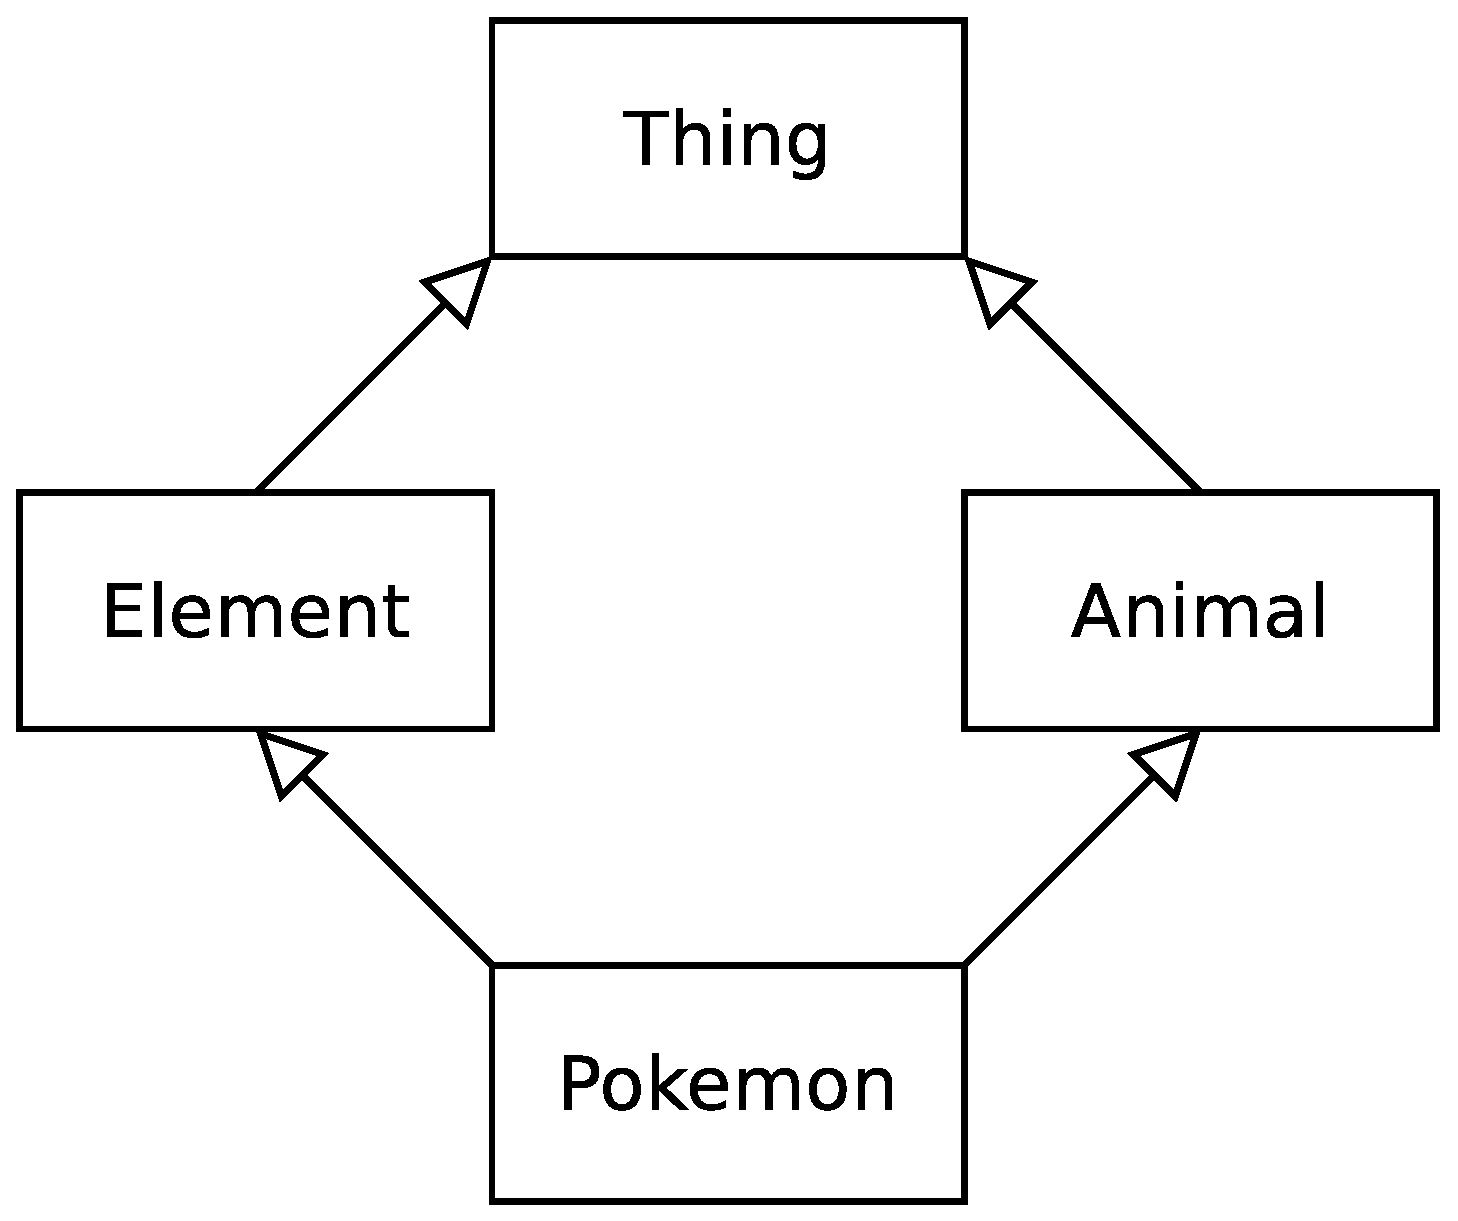
\includegraphics[scale=0.3]{pictures/pokemon}
 \caption{Vererbungshierarchie für die Klasse Pokemon.}
 \label{pokemon}
\end{figure}

Zunächst können wir mit der Klasse Thing sehen, wie eine einfache Klasse definiert wird. Anhand von Thing und den Klassen Element und Animal betrachten wir, wie Felder und Methoden definiert werden können und wie diese vererbt werden.

Schließlich vervollständigen wir die Hierarchie so, dass mit möglichst wenig Klassen möglichst viele Sonderfälle und Probleme abgedeckt werden können. Hierfür eignet sich das Diamond-Problem sehr gut: Eine Klasse, die von zwei Klassen erbt, die wiederum eine gemeinsame Superklasse haben. Element und Animal erben bereits von Thing. Wir nutzen den Umstand also aus und definieren eine Klasse Pokemon, die von beiden erbt.

In jedem Schritt wollen wir betrachten, was passiert, wenn Methoden redefiniert werden, wie disjunkte Mengen von Slots und Methoden vererbt werden, wie mit gleichbenannten Merkmalen umgegangen wird und wie ein Programmierer die Vererbung bei gleichbenannten Merkmalen beeinflussen kann.

Zusätzlich soll beleuchtet werden, welche Möglichkeiten es gibt, Methoden einer Superklasse in einer Subklasse zu ergänzen und ob diese kompatibel mit Mehrfachvererbung sind.